\section{Introducción}

\begin{frame}{El sistema: grúa portacontenedores STS}
  \begin{columns}[T]
    \begin{column}{0.55\textwidth}
      \begin{itemize}
        \item Grúa de muelle tipo pórtico (\textit{Ship-to-Shore}) para carga/descarga de
              contenedores en barcos.
        \item Dos movimientos principales, simultáneos, en un plano vertical (2D):
          \begin{itemize}
            \item \textbf{Carro} (\textit{Trolley}): traslación horizontal.
            \item \textbf{Izaje} (\textit{Hoist}): subida/bajada de la carga.
          \end{itemize}
        \item Carga suspendida que se \textbf{balancea como un péndulo} $\Rightarrow$ ejes
              acoplados.
        \item Objetivo: \textbf{control de accionamientos} y \textbf{operación
              semi-automática coordinada}.
      \end{itemize}
    \end{column}
    \begin{column}{0.45\textwidth}
      \centering
      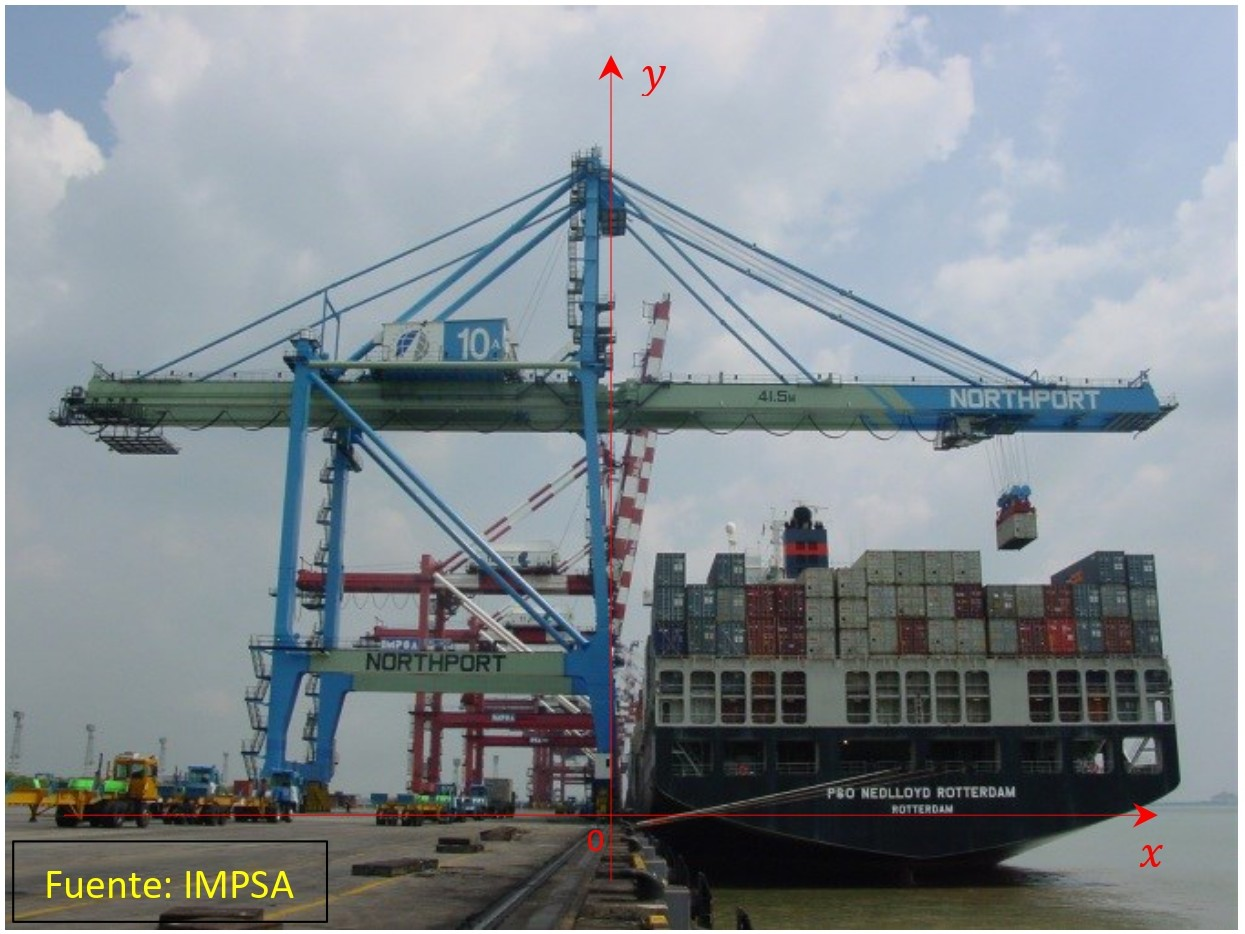
\includegraphics[width=\linewidth]{vista_lateral.jpg}
    \end{column}
  \end{columns}
\end{frame}

\begin{frame}{Arquitectura de control jerárquica}
  \begin{block}{Sistema híbrido de control y protección — 3 niveles}
    \begin{center}
      \begin{tabular}{cll}
        \toprule
        \textbf{Nivel} & \textbf{Rol} & \textbf{Tipo / $T_s$} \\
        \midrule
        \textbf{2} & Regulatorio (torque/velocidad) & Continuo muestreado --- $1$ ms \\
        \textbf{1} & Supervisor (modos, coordinación) & \textbf{Eventos discretos} --- $20$ ms \\
        \textbf{0} & Protección (seguridad) & Eventos discretos --- $20$ ms \\
        \bottomrule
      \end{tabular}
    \end{center}
  \end{block}
  \begin{itemize}
    \item Jerarquía creciente: el Nivel 0 \textbf{sobrescribe} a los superiores ante falla.
    \item La \textbf{planta} (modelo físico y parámetros) es \alert{provista por la cátedra};
          el aporte propio está en el \textbf{diseño de los 3 niveles} y su
          \textbf{implementación}.
  \end{itemize}
\end{frame}
